
\documentclass[12pt]{article}
\usepackage{lingmacros}
\usepackage{tree-dvips}
\usepackage{graphicx}

\usepackage [T2A] {fontenc}   % Кириллица в PDF файле
\usepackage [utf8] {inputenc} % Кодировка текста: utf-8
\usepackage [russian] {babel} % Переносы, лигатуры

\usepackage{graphicx}
\begin{document}

\section{Vision HDL Toolbox}

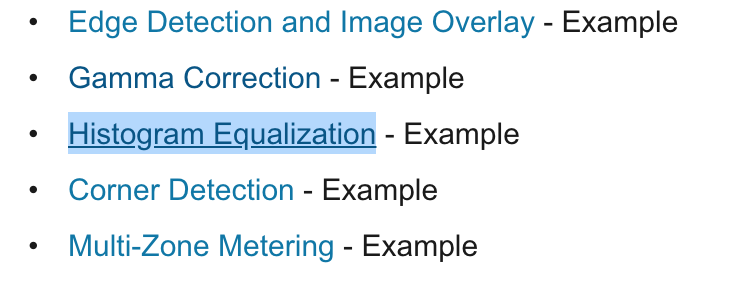
\includegraphics[scale=0.25]{../img/vision_hdl_examples.png}

На рисунке можно посмотреть доступные примеры. Собираются с помощью
еще одного их продукта - HDL Coder. Единственная проблема - хрен воспользуешься
даже триальной версией.

Доступные модули:

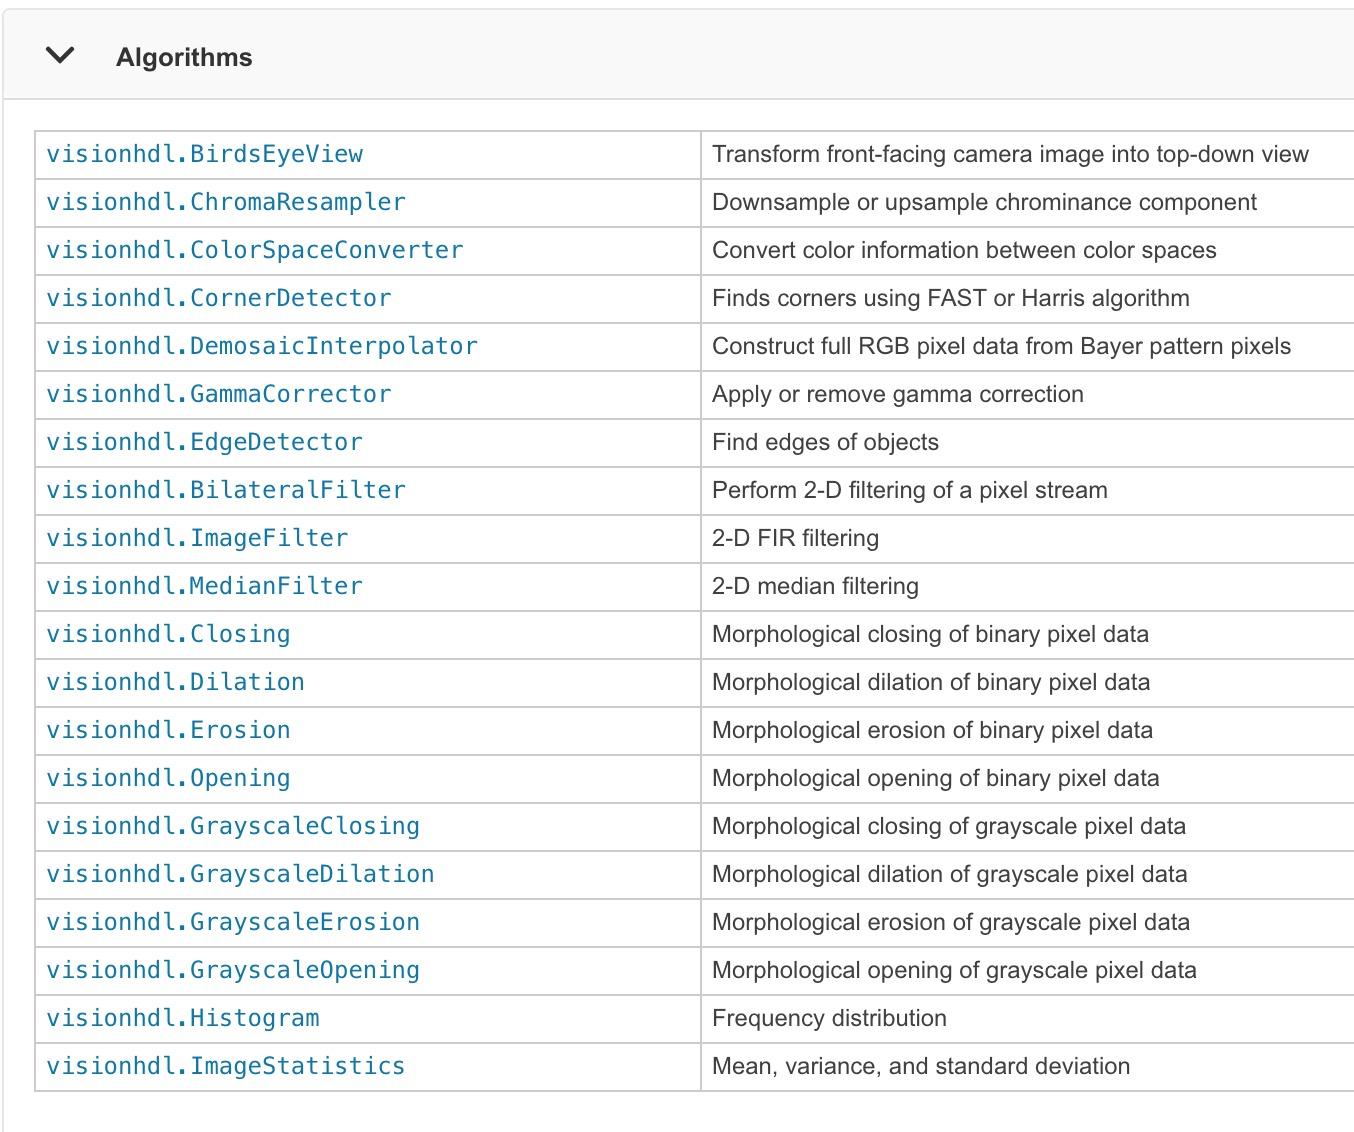
\includegraphics[scale=0.25]{../img/vision_hdl_ip_cores.png}


\section{Xilinx xfOpenCV и HLS}

Выглядит очень интересно, но работает только на Xilinx и только на тех, 
где есть АРМ. Имеет много реализованных функций, а также пишется на C++, 
что несомненно плюс.


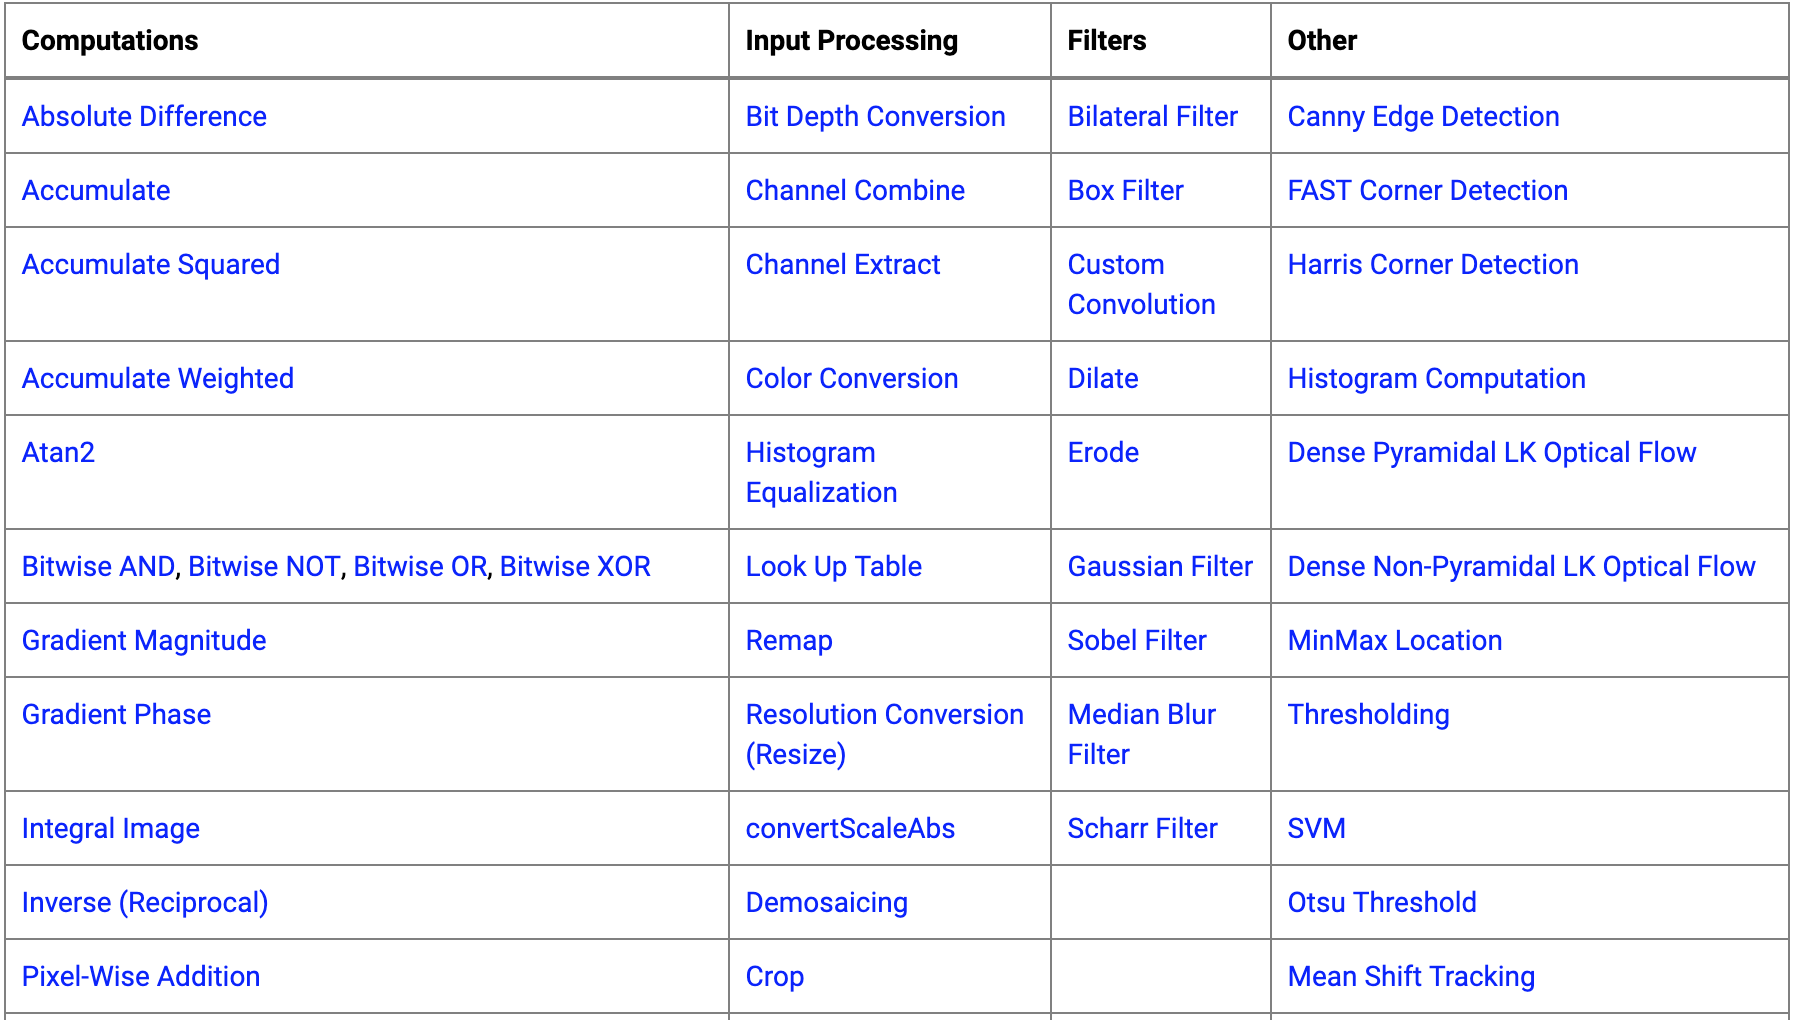
\includegraphics[scale=0.2]{../img/xfopencv2.png}

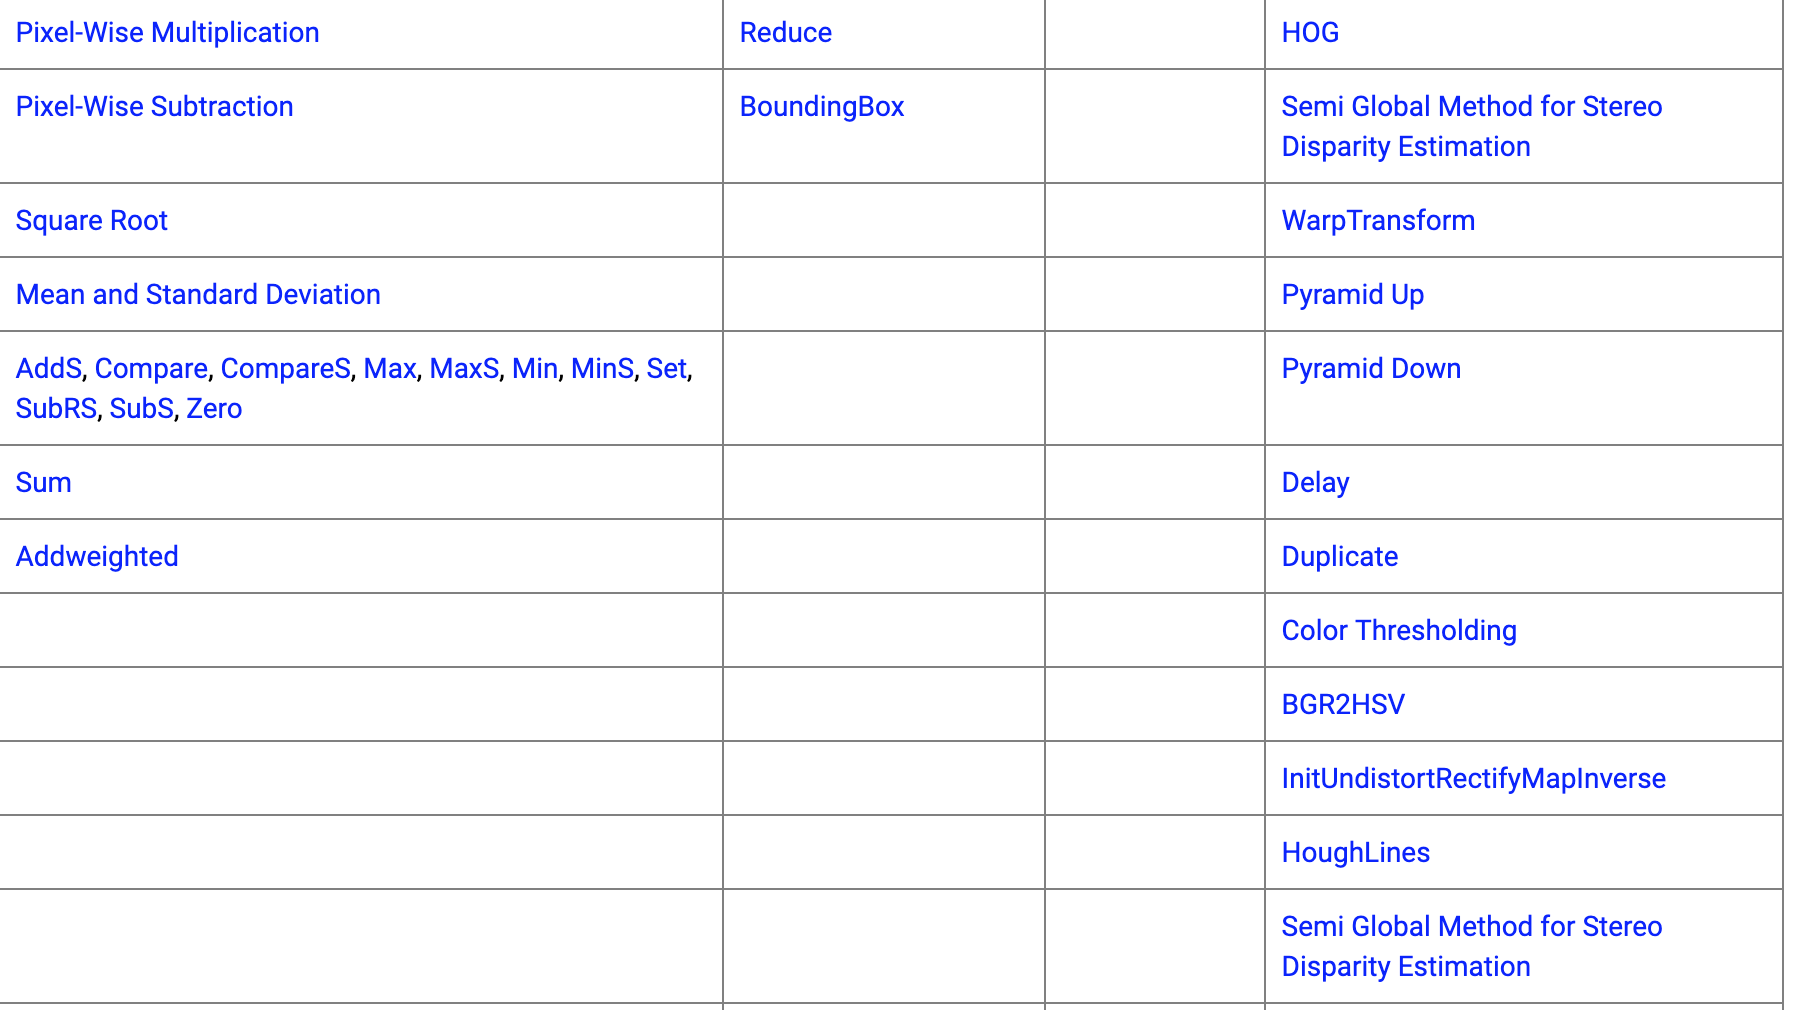
\includegraphics[scale=0.2]{../img/xfopencv1.png}


\section{Lattice IP Cores}
Имеют не очень много IP Cores, зато есть ядра, отвечающие за 
считывание данных с камеры.


\section{OpenCores}

Дамп проектов с OpenCores. Старые, но что-то найти можно.

https://github.com/fabriziotappero/ip-cores


\section{hard-cv}
Куча открытых ip cores для всего на свете.

https://github.com/jpiat/hard-cv


\includegraphics*[scale=.25]{../img/hardcv.png}


\section{Некоторое количество проектов на гите}


\end{document}